Author: Lester Hedges Email:~~ lester.hedges@bristol.ac.uk

\hypertarget{molecular-dynamics}{%
\section{Molecular dynamics}\label{molecular-dynamics}}

The companion notebook for this section can be found
\href{https://github.com/michellab/BioSimSpaceTutorials/blob/4844562e7d2cd0b269cead56562ec16a3dfaef7c/01_introduction/03_molecular_dynamics.ipynb}{here}

\hypertarget{introduction}{%
\subsection{Introduction}\label{introduction}}

In this section we will learn how to use BioSimSpace to configure and
run some basic molecular dynamics simulations.

\hypertarget{protocols}{%
\subsection{Protocols}\label{protocols}}

One of the key goals of BioSimSpace was to start a conversation
regarding \emph{best practice} within the biomolecular simulation
community and to facilitate the codifying of shareable, re-usable, and
extensible simulation protocols.

The
\href{https://biosimspace.org/api/index_Protocol.html}{BioSimSpace.Protocol}
package defines protocols for a range of common molecular dynamics
simulations. We can query the package to ee what protocols are
available:

\begin{Shaded}
\begin{Highlighting}[]
\ImportTok{import}\NormalTok{ BioSimSpace }\ImportTok{as}\NormalTok{ BSS}
\NormalTok{BSS.Protocol.protocols()}
\end{Highlighting}
\end{Shaded}

\begin{verbatim}
['Equilibration',
 'FreeEnergy',
 'Metadynamics',
 'Minimisation',
 'Production',
 'Steering']
\end{verbatim}

Since we require protocols to be \emph{interoperable}, the classes
listed above are simple objects that allow you to configure a
\emph{limited} set of options that are handled by \emph{all} of the
molecular dynamics engines that we support. This might seem quite
restrictive, but we will see later how it is possible to fully customise
a simulation for a particular molecular dynamics engine.

Each protocol comes with some default options. To see what those are we
can instantiate an object using the default constructor. For example,
let's explore the
\href{https://biosimspace.org/api/generated/BioSimSpace.Protocol.Equilibration.html\#BioSimSpace.Protocol.Equilibration}{Equilibration}
protocol.

\begin{Shaded}
\begin{Highlighting}[]
\NormalTok{protocol }\OperatorTok{=}\NormalTok{ BSS.Protocol.Equilibration()}
\BuiltInTok{print}\NormalTok{(protocol)}
\end{Highlighting}
\end{Shaded}

\begin{verbatim}
<BioSimSpace.Protocol.Equilibration: timestep=2.0000 fs, runtime=0.2000 ns, temperature_start=300.0000 K, temperature_end=300.0000 K, pressure=None, report_interval=100, restart_interval=500,restraint=None>
\end{verbatim}

Here we can see that the default protocol performs an equlibration at
fixed temperature (\texttt{temperature\_start\ ==\ temperature\_end}) in
the NVT ensemble (\texttt{pressure=None}) with no restraints
(\texttt{restraint=None}). The total simulation time is 0.2 nanoseconds
with an integration timestep of 2 femtoseconds. The
\texttt{report\_interval} and \texttt{restart\_interval} govern how
frequently information is written to log and restart (and/or trajectory)
files respectively.

If any of these defaults are unsuitable, then you are free to change
them by passing in appropriate values for each of the arguments when
instantiating the object. In some cases it might be desirable to
\emph{override} the default protocols and set specific values of the
arguments that are suitable for a particular project or team. This can
be achieved by defining a set of function wrappers that configure and
return the protocols using your own defaults.

As an example, the following configuration could be used to provide
alternative defaults for NVT and NPT equlibration protocols. (You could
simply re-use the existing protocol name, but here we provide two
separate protocols for convenience.)

\begin{Shaded}
\begin{Highlighting}[]
\CommentTok{# myconfig/Protocol.py}
\ImportTok{import}\NormalTok{ BioSimSpace }\ImportTok{as}\NormalTok{ BSS}

\CommentTok{# Override the equilibration protocol with some custom defaults. Ideally all}
\CommentTok{# arguments to the BioSimSpace function would be mapped, but here we use a}
\CommentTok{# subset for simplicity.}

\CommentTok{# A custom equlibration in the NVT ensemble.}
\KeywordTok{def}\NormalTok{ EquilibrationNVT(runtime}\OperatorTok{=}\DecValTok{5}\OperatorTok{*}\NormalTok{BSS.Units.Time.nanosecond,}
\NormalTok{                     report_interval}\OperatorTok{=}\DecValTok{2500}\NormalTok{,}
\NormalTok{                     restart_interval}\OperatorTok{=}\DecValTok{250000}\NormalTok{,}
\NormalTok{                     restraint}\OperatorTok{=}\StringTok{"backbone"}\NormalTok{):}
    \ControlFlowTok{return}\NormalTok{ BSS.Protocol.Equilibration(runtime}\OperatorTok{=}\NormalTok{runtime,}
\NormalTok{                                      report_interval}\OperatorTok{=}\NormalTok{report_interval,}
\NormalTok{                                      restart_interval}\OperatorTok{=}\NormalTok{restart_interval,}
\NormalTok{                                      restraint}\OperatorTok{=}\NormalTok{restraint)}

\CommentTok{# A custom equlibration in the NPT ensemble.}
\KeywordTok{def}\NormalTok{ EquilibrationNPT(runtime}\OperatorTok{=}\DecValTok{5}\OperatorTok{*}\NormalTok{BSS.Units.Time.nanosecond,}
\NormalTok{                     pressure}\OperatorTok{=}\NormalTok{BSS.Units.Pressure.atm,}
\NormalTok{                     report_interval}\OperatorTok{=}\DecValTok{2500}\NormalTok{,}
\NormalTok{                     restart_interval}\OperatorTok{=}\DecValTok{25000}\NormalTok{,}
\NormalTok{                     restraint}\OperatorTok{=}\StringTok{"backbone"}\NormalTok{):}
    \ControlFlowTok{return}\NormalTok{ BSS.Protocol.Equilibration(runtime}\OperatorTok{=}\NormalTok{runtime,}
\NormalTok{                                      pressure}\OperatorTok{=}\NormalTok{pressure,}
\NormalTok{                                      report_interval}\OperatorTok{=}\NormalTok{report_interval,}
\NormalTok{                                      restart_interval}\OperatorTok{=}\NormalTok{restart_interval,}
\NormalTok{                                      restraint}\OperatorTok{=}\NormalTok{restraint)}
\end{Highlighting}
\end{Shaded}

We could then import the customised protocols from our local
configuraton and use them instead, e.g.:

\begin{Shaded}
\begin{Highlighting}[]
\ImportTok{from}\NormalTok{ myconfig.Protocol }\ImportTok{import} \OperatorTok{*}

\NormalTok{protocol }\OperatorTok{=}\NormalTok{ EquilibrationNVT()}
\BuiltInTok{print}\NormalTok{(protocol)}
\end{Highlighting}
\end{Shaded}

\begin{verbatim}
<BioSimSpace.Protocol.Equilibration: timestep=2.0000 fs, runtime=5.0000 ns, temperature_start=300.0000 K, temperature_end=300.0000 K, pressure=None, report_interval=2500, restart_interval=250000,restraint='backbone'>
\end{verbatim}

\hypertarget{processes}{%
\subsection{Processes}\label{processes}}

Once you have created a molecular system and chosen a protocol, then it
is time to create a simulation \emph{process}. The
\href{https://biosimspace.org/api/index_Process.html}{BioSimSpace.Process}
package provides functionality for configuring and running processes
with several common molecular dynamics engines.

Let's query the package to see what engines are available:

\begin{Shaded}
\begin{Highlighting}[]
\NormalTok{BSS.Process.engines()}
\end{Highlighting}
\end{Shaded}

\begin{verbatim}
['Amber', 'Gromacs', 'Namd', 'OpenMM', 'Somd']
\end{verbatim}

Before creating a process let us once again load our example
alanine-dipeptide system from file:

\begin{Shaded}
\begin{Highlighting}[]
\NormalTok{system }\OperatorTok{=}\NormalTok{ BSS.IO.readMolecules(}\StringTok{"inputs/ala*"}\NormalTok{)}
\end{Highlighting}
\end{Shaded}

As a simple example, let us use a short minimisation protocol:

\begin{Shaded}
\begin{Highlighting}[]
\NormalTok{protocol }\OperatorTok{=}\NormalTok{ BSS.Protocol.Minimisation(steps}\OperatorTok{=}\DecValTok{1000}\NormalTok{)}
\end{Highlighting}
\end{Shaded}

We'll now create a process to apply the \texttt{Protocol} to the
\texttt{System} using the AMBER molecular dynamics engine:

\begin{Shaded}
\begin{Highlighting}[]
\NormalTok{process }\OperatorTok{=}\NormalTok{ BSS.Process.Amber(system, protocol)}
\end{Highlighting}
\end{Shaded}

A lot of complexity is hidden in this line. BioSimSpace has
automatically found an AMBER executable on the underlying operating
system, has automatically written AMBER format molecular input files,
generated an AMBER configuration file for the minimisation protocol, and
configured any command-line arguments that are required.

By default, processes are run inside of a temporary working directory
hidden away from the user. To see where this is, run:

\begin{Shaded}
\begin{Highlighting}[]
\NormalTok{process.workDir()}
\end{Highlighting}
\end{Shaded}

\begin{verbatim}
'/tmp/tmpjuzioj_o'
\end{verbatim}

N.B. If you want to use a different temporary directory, e.g.~one with a
faster disk, then simply set the \texttt{TMPDIR} environment variable.
Alternatively, you can pass the \texttt{work\_dir} argument to the
\texttt{Process} constructor to explicitly specify the path. This can be
useful when you want named directories, or want to examine the
intermediate files from the \texttt{Process} for debugging purposes.

To see what executable was found, run:

\begin{Shaded}
\begin{Highlighting}[]
\NormalTok{process.exe()}
\end{Highlighting}
\end{Shaded}

\begin{verbatim}
'/home/lester/sire.app/bin/sander'
\end{verbatim}

To see the list of autogenerated input files:

\begin{Shaded}
\begin{Highlighting}[]
\NormalTok{process.inputFiles()}
\end{Highlighting}
\end{Shaded}

\begin{verbatim}
['/tmp/tmpjuzioj_o/amber.cfg',
 '/tmp/tmpjuzioj_o/amber.rst7',
 '/tmp/tmpjuzioj_o/amber.prm7']
\end{verbatim}

If you like, we could zip up the input files to use on another occasion.
When working on a notebook server it's possible to return a file link so
that we can download them:

\begin{Shaded}
\begin{Highlighting}[]
\NormalTok{process.getInput(file_link}\OperatorTok{=}\VariableTok{True}\NormalTok{)}
\end{Highlighting}
\end{Shaded}

amber\_input.zip

We can query also query the list of configuration file options:

\begin{Shaded}
\begin{Highlighting}[]
\NormalTok{process.getConfig()}
\end{Highlighting}
\end{Shaded}

\begin{verbatim}
['Minimisation',
 ' &cntrl',
 '  imin=1,',
 '  ntx=1,',
 '  ntxo=1,',
 '  ntpr=100,',
 '  irest=0,',
 '  maxcyc=1000,',
 '  ncyc=1000,',
 '  cut=8.0,',
 ' /']
\end{verbatim}

And also get command-line argument string for the process:

\begin{Shaded}
\begin{Highlighting}[]
\NormalTok{process.getArgString()}
\end{Highlighting}
\end{Shaded}

\begin{verbatim}
'-O -i amber.cfg -p amber.prm7 -c amber.rst7 -o stdout -r amber.crd -inf amber.nrg'
\end{verbatim}

If you're an expert in a particular package then BioSimSpace allows you
to fully customise the process by tweaking the configuration options and
command-line arguments. Read the help documentation for
\texttt{process.setConfig} and \texttt{process.setArgs} if you are
interested. Once again, it's possible to wrap the instantiation of
\texttt{Process} objects in your own custom functions, allowing you to
tweak the default configuration options for your own requirements. For
example, if you always want to wrap coordinates to the minimum image
when using AMBER, then this could be achieved as follows:

\begin{Shaded}
\begin{Highlighting}[]
\CommentTok{# myconfig/Process.py}
\ImportTok{import}\NormalTok{ BioSimSpace }\ImportTok{as}\NormalTok{ BSS}

\CommentTok{# Wrap the instantiation of BSS.Process.Amber objects to configure them}
\CommentTok{# such that coordinates are always wrapped to the minimum image.}
\KeywordTok{def}\NormalTok{ Amber(system, protocol, exe}\OperatorTok{=}\VariableTok{None}\NormalTok{, name}\OperatorTok{=}\StringTok{"amber"}\NormalTok{,}
\NormalTok{            work_dir}\OperatorTok{=}\VariableTok{None}\NormalTok{, seed}\OperatorTok{=}\VariableTok{None}\NormalTok{, property_map}\OperatorTok{=}\NormalTok{\{\}):}

    \CommentTok{# Create process using the passed parameters.}
\NormalTok{    process }\OperatorTok{=}\NormalTok{ BSS.Process.Amber(system,}
\NormalTok{                                protocol,}
\NormalTok{                                exe}\OperatorTok{=}\NormalTok{exe,}
\NormalTok{                                name}\OperatorTok{=}\NormalTok{name,}
\NormalTok{                                work_dir}\OperatorTok{=}\NormalTok{work_dir,}
\NormalTok{                                seed}\OperatorTok{=}\NormalTok{seed,}
\NormalTok{                                property_map}\OperatorTok{=}\NormalTok{property_map)}
    
    \CommentTok{# Get the config.}
\NormalTok{    config }\OperatorTok{=}\NormalTok{ process.getConfig()}
    
    \CommentTok{# Add coordinate wrapping to the end of the config.}
\NormalTok{    config[}\OperatorTok{-}\DecValTok{1}\NormalTok{] }\OperatorTok{=} \StringTok{"  iwrap=1,"}
\NormalTok{    config.append(}\StringTok{" /"}\NormalTok{)}

    \CommentTok{# Set the new config.}
\NormalTok{    process.setConfig(config)}
    
    \CommentTok{# Return the process.}
    \ControlFlowTok{return}\NormalTok{ process}
\end{Highlighting}
\end{Shaded}

Let us know create our custom AMBER process and check the configuration:

\begin{Shaded}
\begin{Highlighting}[]
\ImportTok{from}\NormalTok{ myconfig.Process }\ImportTok{import} \OperatorTok{*}

\NormalTok{process }\OperatorTok{=}\NormalTok{ Amber(system, protocol)}
\NormalTok{process.getConfig()}
\end{Highlighting}
\end{Shaded}

\begin{verbatim}
['Minimisation',
 ' &cntrl',
 '  imin=1,',
 '  ntx=1,',
 '  ntxo=1,',
 '  ntpr=100,',
 '  irest=0,',
 '  maxcyc=1000,',
 '  ncyc=1000,',
 '  cut=8.0,',
 '  iwrap=1,',
 ' /']
\end{verbatim}

N.B. You might want to add additional configuration details to your
\texttt{Process} wrappers, e.g.~to ensure that a specific executable is
used.

Now that we have a process, let's go ahead and start it:

\begin{Shaded}
\begin{Highlighting}[]
\NormalTok{process.start()}
\end{Highlighting}
\end{Shaded}

\begin{verbatim}
BioSimSpace.Process.Amber(<BioSimSpace.System: nMolecules=631>, <BioSimSpace.Protocol.Custom>, exe='/home/lester/sire.app/bin/sander', name='amber', work_dir='/tmp/tmpm8kx_jms', seed=None)
\end{verbatim}

BioSimSpace has now launched a minimisation process in the background!
When in an interactive session you carry on working and periodically
check in on the process to see how its doing.

To check whether the process is running:

\begin{Shaded}
\begin{Highlighting}[]
\NormalTok{process.isRunning()}
\end{Highlighting}
\end{Shaded}

\begin{verbatim}
True
\end{verbatim}

We can see how many minutes it has been running for:

\begin{Shaded}
\begin{Highlighting}[]
\NormalTok{process.runTime()}
\end{Highlighting}
\end{Shaded}

\begin{verbatim}
0.1960 mins
\end{verbatim}

Since this is a short minimisation it will likely finish pretty quickly.
Let's print the final energy of the system and return the minimised
molecular configuration.

\begin{Shaded}
\begin{Highlighting}[]
\BuiltInTok{print}\NormalTok{(process.getTotalEnergy(block}\OperatorTok{=}\VariableTok{True}\NormalTok{))}
\NormalTok{minimised }\OperatorTok{=}\NormalTok{ process.getSystem()}
\end{Highlighting}
\end{Shaded}

\begin{verbatim}
-6954.7000 kcal/mol
\end{verbatim}

When working interactively, any time we query a running process we get
back the \emph{latest} information that has been written to disk. This
means that we can get an update on how things are progressing, then
immediately carry on with what we were doing in our notebook. By passing
\texttt{block=True}, as we do when we call \texttt{getTotalEnergy}
above, we request that the process finishes running before returning a
result. This means we get the \emph{final} energy, and the minimised
system that is returned afterwards represents the \emph{final} snapshot
that was saved.

Let's now re-run the simulation, instead using GROMACS as the MD engine.

\begin{Shaded}
\begin{Highlighting}[]
\NormalTok{process }\OperatorTok{=}\NormalTok{ BSS.Process.Gromacs(system, protocol)}
\end{Highlighting}
\end{Shaded}

When the process is instantiated, BioSimSpace takes the system that was
read from AMBER format files and converts it to GROMACS format ready for
simulation. Let's take a look at the list of input files that were
autogenerated for us:

\begin{Shaded}
\begin{Highlighting}[]
\NormalTok{process.inputFiles()}
\end{Highlighting}
\end{Shaded}

\begin{verbatim}
['/tmp/tmpsxf5hoej/gromacs.mdp',
 '/tmp/tmpsxf5hoej/gromacs.gro',
 '/tmp/tmpsxf5hoej/gromacs.top',
 '/tmp/tmpsxf5hoej/gromacs.tpr']
\end{verbatim}

Let's start the process running and, once again, wait for it to finish
before getting the minimised system.

\begin{Shaded}
\begin{Highlighting}[]
\NormalTok{process.start()}
\NormalTok{minimised }\OperatorTok{=}\NormalTok{ process.getSystem(block}\OperatorTok{=}\VariableTok{True}\NormalTok{)}
\end{Highlighting}
\end{Shaded}

\hypertarget{interactive-molecular-dynamics}{%
\subsection{Interactive molecular
dynamics}\label{interactive-molecular-dynamics}}

The example in the previous section was finished almost as soon as it
began. Let's run a more complicated equilibration protocol so that we
can learn more about how to monitor processes interactively using
BioSimSpace.

\begin{Shaded}
\begin{Highlighting}[]
\NormalTok{protocol }\OperatorTok{=}\NormalTok{ BSS.Protocol.Equilibration(runtime}\OperatorTok{=}\DecValTok{20}\OperatorTok{*}\NormalTok{BSS.Units.Time.picosecond,}
\NormalTok{                                      temperature_start}\OperatorTok{=}\DecValTok{0}\OperatorTok{*}\NormalTok{BSS.Units.Temperature.kelvin,}
\NormalTok{                                      temperature_end}\OperatorTok{=}\DecValTok{300}\OperatorTok{*}\NormalTok{BSS.Units.Temperature.kelvin,}
\NormalTok{                                      restraint}\OperatorTok{=}\StringTok{"backbone"}\NormalTok{)}
\end{Highlighting}
\end{Shaded}

This protocol will equlibrate a system for 20 picoseconds, while heating
it from 0 to 300 Kelvin and restraining any atoms in the backbone of the
molecule. Note that some of the parameters passed have units, e.g.~the
temperatures are in Kelvin. BioSimSpace has a built in type system for
handling variables with units. The \texttt{BSS.Units} package provides a
convenient way of declaring these, for example
\texttt{10*BSS.Units.Temperature.kelvin} creates an object of type
\texttt{BSS.Types.Temperature} with a magnitude of 10 and unit of
Kelvin. This allows the user to pass parameters with whatever unit they
like. BioSimSpace will simply convert it to the correct unit for the
chosen MD engine internally.

One again, we now need a \texttt{Process} in order to run our
simulation. Exectute the cell below to initialise an AMBER process and
start it immediately. Note that we pass in the minimised system from the
last example, along with our new protocol.

\begin{Shaded}
\begin{Highlighting}[]
\NormalTok{process }\OperatorTok{=}\NormalTok{ BSS.Process.Amber(minimised, protocol).start()}
\end{Highlighting}
\end{Shaded}

We can monitor the time, temperature, and energy as the process runs. If
you run this multiple times using ``CTRL+Return'' you'll see the
temperature slowly increasing.

\begin{Shaded}
\begin{Highlighting}[]
\BuiltInTok{print}\NormalTok{(process.getTime(), process.getTemperature(), process.getTotalEnergy())}
\end{Highlighting}
\end{Shaded}

\begin{verbatim}
2.4000 ps 30.6900 K -6936.6583 kcal/mol
\end{verbatim}

Since all of the values returned above are typed we can easily convert
them to other units:

\begin{Shaded}
\begin{Highlighting}[]
\BuiltInTok{print}\NormalTok{(process.getTime().nanoseconds(), process.getTemperature().celsius(), process.getTotalEnergy().kj_per_mol())}
\end{Highlighting}
\end{Shaded}

\begin{verbatim}
0.0050 ns -204.7600 C -2.7995e+04 kJ/mol
\end{verbatim}

It's possible to query many other thermodynamic records. What's
available depends on type of protocol and the MD package that is used to
run the protocol. To get more information, run:

N.B. Certain functionality is specific to the process in question, i.e.
\texttt{BSS.Process.Amber} will have different options to
\texttt{BSS.Process.Gromacs}, but, for the purposes of interoperability,
there is a core set of functionality that is consistent across all
\texttt{Process} classes, e.g.~all classes implement a
\texttt{getSystem} method.)

\hypertarget{plotting-time-series-data}{%
\subsubsection{Plotting time series
data}\label{plotting-time-series-data}}

As well as querying the most recent records we can also get a time
series of results by passing the \texttt{time\_series} keyword argument
to any of the data record getter methods, e.g.

\begin{Shaded}
\begin{Highlighting}[]
\CommentTok{# Get a time series of pressure records.}
\NormalTok{pressure }\OperatorTok{=}\NormalTok{ process.getPressure(time_series}\OperatorTok{=}\VariableTok{True}\NormalTok{)}
\end{Highlighting}
\end{Shaded}

The \texttt{BSS.Notebook} package provides several useful tools that are
available when working inside of a Jupyter notebook. One of these is the
plot function, that allows us to create simple x/y plots of time-series
data.

Let's grab the same record data as above and use it to make some graphs
of the data.

\begin{Shaded}
\begin{Highlighting}[]
\CommentTok{# Generate a plot of time vs temperature.}
\NormalTok{plot1 }\OperatorTok{=}\NormalTok{ BSS.Notebook.plot(process.getTime(time_series}\OperatorTok{=}\VariableTok{True}\NormalTok{), process.getTemperature(time_series}\OperatorTok{=}\VariableTok{True}\NormalTok{))}

\CommentTok{# Generate a plot of time vs energy.}
\NormalTok{plot2 }\OperatorTok{=}\NormalTok{ BSS.Notebook.plot(process.getTime(time_series}\OperatorTok{=}\VariableTok{True}\NormalTok{), process.getTotalEnergy(time_series}\OperatorTok{=}\VariableTok{True}\NormalTok{))}
\end{Highlighting}
\end{Shaded}

\begin{figure}
\centering
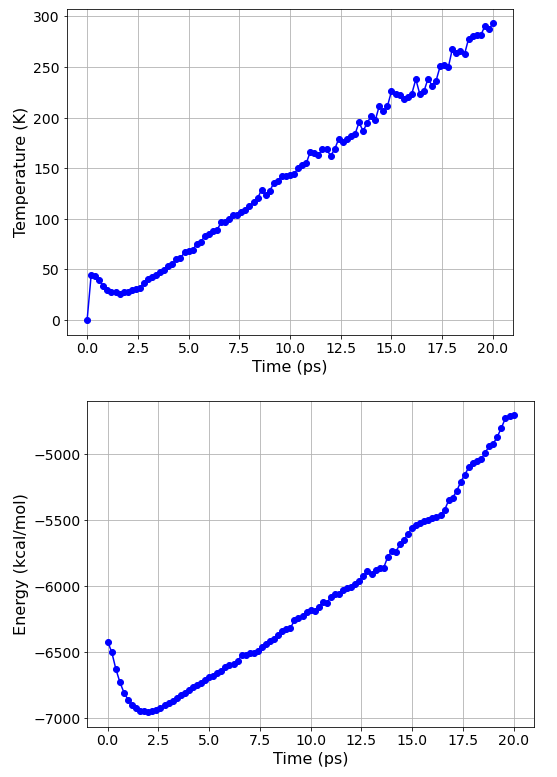
\includegraphics{https://github.com/michellab/BioSimSpaceTutorials/blob/dd5a24e58778af21612ade7febe5ba7fd98f9885/01_introduction/assets/03_time_series.png}
\caption{Time-series plots}
\end{figure}

(Note that, by default, the axis labels axis labels are automatically
generated from the types and units of the x and y data that are passed
to the function.)

Re-run the cell using ``CTRL+Return'' to see the graphs update as the
simulation progesses. (Occasionally, you might see a warning that the x
and y data sets are mismatched in length, this is because the data was
extracted before all records were written to disk.)

Being able to query a process in real time is an incredibly useful tool.
This could enable us to check for convergence, or spot errors in the
simulation. If you ever need to kill a running process (perhaps it was
configured incorrectly), run:

\begin{Shaded}
\begin{Highlighting}[]
\NormalTok{process.kill()}
\end{Highlighting}
\end{Shaded}

\hypertarget{visualising-the-molecular-system}{%
\subsubsection{Visualising the molecular
system}\label{visualising-the-molecular-system}}

Another useful tool that is available when working inside of a notebook
is the \texttt{View} class that can be used to visualise the molecular
system while a process is running. To create a \texttt{View} object we
must attach it to a process (or a molecular system), e.g.:

\begin{Shaded}
\begin{Highlighting}[]
\NormalTok{view }\OperatorTok{=}\NormalTok{ BSS.Notebook.View(process)}
\end{Highlighting}
\end{Shaded}

We can now visualise the system:

\begin{Shaded}
\begin{Highlighting}[]
\NormalTok{view.system()}
\end{Highlighting}
\end{Shaded}

\begin{figure}
\centering
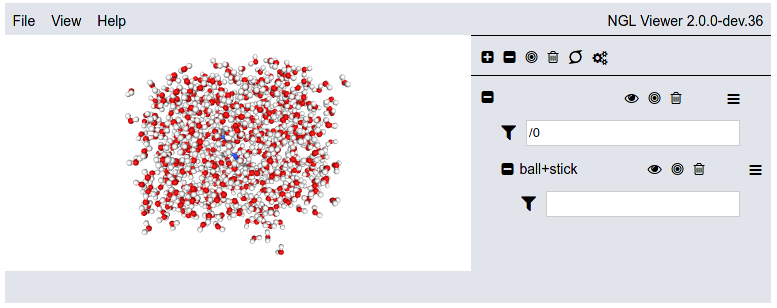
\includegraphics{https://github.com/michellab/BioSimSpaceTutorials/blob/dd5a24e58778af21612ade7febe5ba7fd98f9885/01_introduction/assets/03_view_system.png}
\caption{Visualise the system}
\end{figure}

(If you see an empty view, try re-executing the cell.)

To only view a specific molecule:

\begin{Shaded}
\begin{Highlighting}[]
\NormalTok{view.molecule(}\DecValTok{0}\NormalTok{)}
\end{Highlighting}
\end{Shaded}

\begin{figure}
\centering
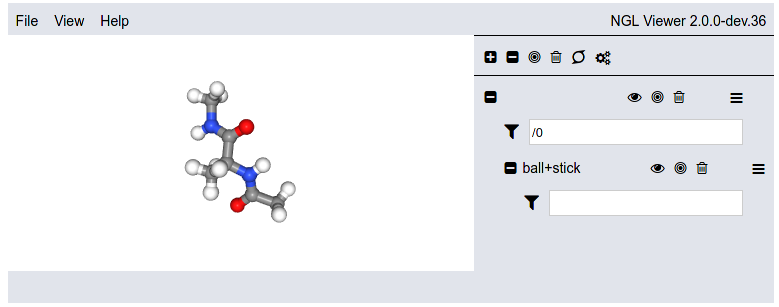
\includegraphics{https://github.com/michellab/BioSimSpaceTutorials/blob/86442df77e2ad33ae79f62e214a53af42cb320ec/01_introduction/assets/03_view_molecule.png}
\caption{Visualise a molecule}
\end{figure}

To view a list of molecules:

\begin{Shaded}
\begin{Highlighting}[]
\NormalTok{view.molecules([}\DecValTok{0}\NormalTok{, }\DecValTok{5}\NormalTok{, }\DecValTok{10}\NormalTok{])}
\end{Highlighting}
\end{Shaded}

\begin{figure}
\centering
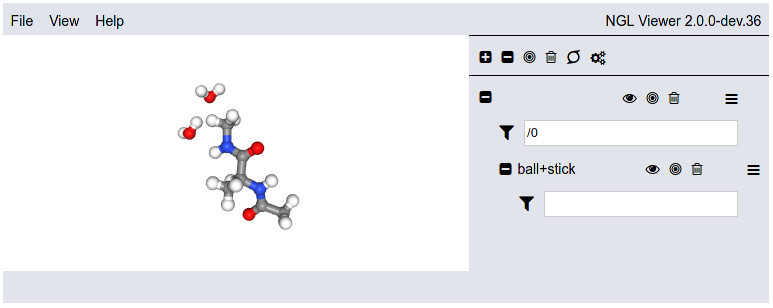
\includegraphics{https://github.com/michellab/BioSimSpaceTutorials/blob/86442df77e2ad33ae79f62e214a53af42cb320ec/01_introduction/assets/03_view_molecules.png}
\caption{Visualise some molecules}
\end{figure}

If a particular view was of interest it can be reloaded as follows:

\begin{Shaded}
\begin{Highlighting}[]
\CommentTok{# Reload the original view.}
\NormalTok{view.}\BuiltInTok{reload}\NormalTok{(}\DecValTok{0}\NormalTok{)}
\end{Highlighting}
\end{Shaded}

\begin{figure}
\centering
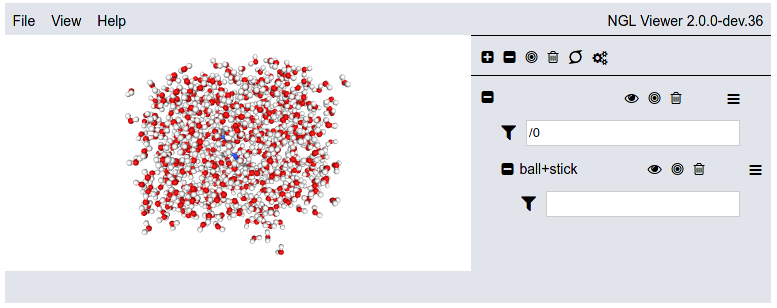
\includegraphics{https://github.com/michellab/BioSimSpaceTutorials/blob/dd5a24e58778af21612ade7febe5ba7fd98f9885/01_introduction/assets/03_view_system.png}
\caption{Visualise the system}
\end{figure}

To save a specific view as a PDB file:

\begin{Shaded}
\begin{Highlighting}[]
\NormalTok{view.savePDB(}\StringTok{"my_view.pdb"}\NormalTok{, index}\OperatorTok{=}\DecValTok{0}\NormalTok{)}
\end{Highlighting}
\end{Shaded}

\hypertarget{reading-and-analysing-trajectory-data}{%
\subsubsection{Reading and analysing trajectory
data¶}\label{reading-and-analysing-trajectory-data}}

The \texttt{BSS.Trajectory} package comes with a set of tools for
reading and analysis trajectory files. Files can be loaded directly, or
if supported, can be read from a running process.

For example, to get the trajectory from the process, run:

\begin{Shaded}
\begin{Highlighting}[]
\NormalTok{traj }\OperatorTok{=}\NormalTok{ process.getTrajectory()}
\end{Highlighting}
\end{Shaded}

(If you get an error, then the trajectory file may be in the process of
being written. Simply try again.)

To get the current number of frames:

\begin{Shaded}
\begin{Highlighting}[]
\NormalTok{traj.nFrames()}
\end{Highlighting}
\end{Shaded}

\begin{verbatim}
20
\end{verbatim}

To get all of the frames as a list of \texttt{System} objects:

\begin{Shaded}
\begin{Highlighting}[]
\NormalTok{frames }\OperatorTok{=}\NormalTok{ traj.getFrames()}
\end{Highlighting}
\end{Shaded}

Specific frames can be extracted by passing a list of indices, e.g.~the
first and last:

\begin{Shaded}
\begin{Highlighting}[]
\NormalTok{frames }\OperatorTok{=}\NormalTok{ traj.getFrames([}\DecValTok{0}\NormalTok{, }\DecValTok{-1}\NormalTok{])}
\end{Highlighting}
\end{Shaded}

Like most things in BioSimSpace, the \texttt{Trajectory} class is simply
a wrapper around existing tools. Internally, trajectories are stored as
an \href{http://mdtraj.org}{MDTraj} object. This can be obtained,
allowing the user direct access to the full power of MDTraj:

\begin{Shaded}
\begin{Highlighting}[]
\NormalTok{mdtraj }\OperatorTok{=}\NormalTok{ traj.getTrajectory()}
\BuiltInTok{type}\NormalTok{(mdtraj)}
\end{Highlighting}
\end{Shaded}

\begin{verbatim}
mdtraj.core.trajectory.Trajectory
\end{verbatim}

Alternatively, a trajectory can be returned in
\href{https://www.mdanalysis.org}{MDAnalysis} format:

\begin{Shaded}
\begin{Highlighting}[]
\NormalTok{mdanalysis }\OperatorTok{=}\NormalTok{ traj.getTrajectory(}\BuiltInTok{format}\OperatorTok{=}\StringTok{"mdanalysis"}\NormalTok{)}
\BuiltInTok{type}\NormalTok{(mdanalysis)}
\end{Highlighting}
\end{Shaded}

\begin{verbatim}
MDAnalysis.core.universe.Universe
\end{verbatim}

The \texttt{Trajectory} class also provides wrappers around some basic
MDTraj analysis tools, allowing the user to compute quantities such as
the root mean squared displacement (RMSD).

Let's measure the RMSD of the alanine-dipeptide molecule with a
reference to its configuration in the first trajectory frame. To extract
the alanine-dipeptide, we search the system for a residue named ALA.
We'll also plot the RMSD for each frame of the trajectory.

\begin{Shaded}
\begin{Highlighting}[]
\CommentTok{# Search the system for a residue named ALA. Since there is a single match,}
\CommentTok{# we take the first result.}
\NormalTok{molecule }\OperatorTok{=}\NormalTok{ system.search(}\StringTok{"mol with resname ALA"}\NormalTok{)[}\DecValTok{0}\NormalTok{]}

\CommentTok{# Get the indices of the atoms in the molecule, relative to the original system.}
\NormalTok{indices }\OperatorTok{=}\NormalTok{ [system.getIndex(x) }\ControlFlowTok{for}\NormalTok{ x }\KeywordTok{in}\NormalTok{ molecule.getAtoms()]}

\CommentTok{# Compute the RMSD for each frame and plot the result.}
\NormalTok{BSS.Notebook.plot(y}\OperatorTok{=}\NormalTok{process.getTrajectory().rmsd(frame}\OperatorTok{=}\DecValTok{0}\NormalTok{, atoms}\OperatorTok{=}\NormalTok{indices),}
\NormalTok{                  xlabel}\OperatorTok{=}\StringTok{"Frame"}\NormalTok{, ylabel}\OperatorTok{=}\StringTok{"RMSD"}\NormalTok{)}
\end{Highlighting}
\end{Shaded}

\begin{figure}
\centering
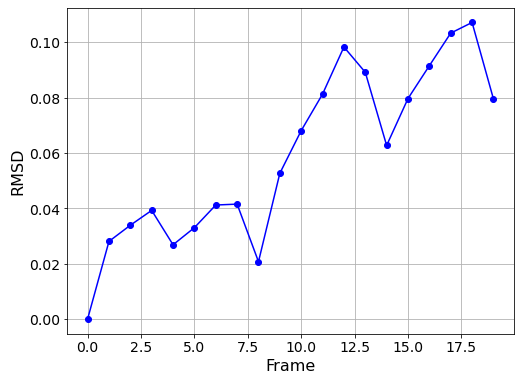
\includegraphics{https://github.com/michellab/BioSimSpaceTutorials/blob/dd5a24e58778af21612ade7febe5ba7fd98f9885/01_introduction/assets/03_rmsd.png}
\caption{RMSD vs frame index}
\end{figure}
